\documentclass[11pt]{report}
\usepackage{fullpage}

\usepackage{graphics}
\usepackage{graphicx}
\usepackage{float}
\usepackage[normalem]{ulem}
\usepackage{framed}

\title{\LaTeX{} for Newbies}
\author {Anish Kumar Mishra}
\date{\today}
\begin{document}
\maketitle
\tableofcontents

\chapter{Introduction}

\LaTeX{} is a typesetting program used widely in scientific community to prepare documents. It allows the user to typeset their content using tags and formatting commands.
There are several features provided by this program, some of them are typesetting, cross-referencing, embedding tables and images inside documents, etc.


\subsection{Why \LaTeX{}?} \label{ew}

A simple question one may ask that why we need yet another document preparation tool when we have so many 
of them like MS Word already available in the market. The answer to this is that \LaTeX{} comes free of cost 
and the time it takes to prepare a large document is very less. Also using \LaTeX{} enables you to have more finer control over 
the appearence of your document.

\chapter{Getting Started}

There are some simple steps you need to follow in order to get started. It is assumed that you are trying to prepare your document on a linux system.
The steps are: 
\begin{enumerate}
  \item Open an editor of your choice(Kile or Vim).
  \item Write the following commands as shown in the figure \ref{fig1}
  \item Save the file with a .tex extension.
  \item Type the command pdflatex at your terminal.
  \item A pdf will be generated in the same folder as your .tex file.
      \begin{figure}[H]
	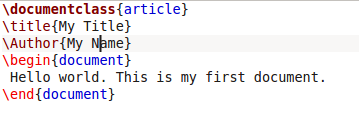
\includegraphics[width=7cm, height=3cm]{screen/shot1}
	\caption{A Simple \LaTeX{} Document}
	\label{fig1}
      \end{figure}
 \end{enumerate} 
In the above example \begin{verbatim} \documentclass, \begin, etc. \end{verbatim} 
are the commands and everything inside \verb|{..}| are the arguments to the command. 
this document will cover brief description of the commands and their usage.


\chapter{Document Types}

\LaTeX{} documents starts with \verb|\documentclass{class}| and end with 
\verb|\end{document}.|

\noindent Some of the well known and widely used classes are as given in table below.

\begin{table}[htb]
\caption{Document class}
\begin{tabular} {|c|l|}
\hline
{\bf Class} & {\bf Description} \\ 
\hline \hline article & for articles in scientific journals, presentations, short reports, program documentations,...\\
\hline report & for longer reports containing several chapters, small books, thesis, ... \\
\hline book & for real books \\
\hline slides & for slides \\
\hline letter & for writting letters. \\
\hline
\end{tabular}
\end{table}


\chapter {Inserting Pictures}
To insert a picture in your document use \verb|\begin{figure} and \end{figure}.| 
An example for this is shown below in figure\ref{fig2}.
\hspace{3mm}
\begin{figure}[H]
  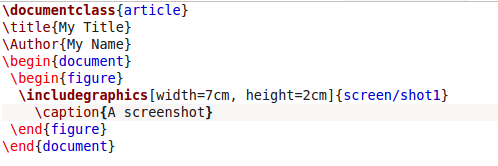
\includegraphics[width=10cm, height=3cm]{screen/shot2}
  \caption{Basic commands for figure}
  \label{fig2}
\end{figure}

Also note that you should include the package \verb|\usepackage{graphics}, \usepackage{graphicx}| 
at the beginning of your document.
\hspace{3mm}


\chapter {Working With Tables}
If you want a table in your document then you need to use \verb|\begin{tabular} and \end{tabular}| 
commands. 
A sample code is shown below in figure\ref{fig3}.

\begin{figure}[H]
  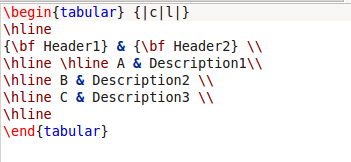
\includegraphics[width=10cm, height=3cm]{screen/shot3}
  \caption{Basic commands for table}
  \label{fig3}
\end{figure}

\chapter{Working With List Of Items}
The two most commonly used list items - Numbered List and Bulleted List can be created using \LaTeX\ as shown below.

\subsection{Numbered List}
A numbered list can be created in \LaTeX\ using the tags as-
\begin{verbatim}
\begin{enumerate}
\item SSC
\item HSC
\item Graduation
\item Post-Graduation
\item Doctorate
\item Post-Doctorate
\end{enumerate}
\end{verbatim}
And the above command will give the ouput as shown below -
\begin{enumerate}
\item SSC
\item HSC
\item Graduation
\item Post-Graduation
\item Doctorate
\item Post-Doctorate
\end{enumerate}

\subsection{Bulleted List}
A bulleted list can be created in \LaTeX\ using the tags as-
\begin{verbatim}
\begin{itemize}
\item Hollywood
\item Bollywood
\item Tollywood
\item Kollywood
\end{itemize}
\end{verbatim}
And the above command will give the ouput as shown below -

\begin{itemize}
\item Hollywood
\item Bollywood
\item Tollywood
\item Kollywood
\end{itemize}

\chapter{Styling The Text}
Some part of text can be formatted in special ways. Below are the few \LaTeX\ commands used for the purpose.
\vspace{3mm}

\begin{tabular} {l l l}

 \verb| \textit{...} | & \textit{italic} & Italicizes the text. These are used for emphasis\\
 \verb| \textsc{...} | & \textsc{Small Cap} &  Used for Small Cap heading or may be used in text \\
 \verb| \textbf{...} | & \textbf{Bold Face} & Bold face are used in text for emphasis a word in text \\
 \verb| \textsf{...} | & \textsf{Sans Serif} & Required for Sans Serif font \\
 \verb| \texttt{...} | & \texttt{typewriter} & These are used when typewriter font is required \\
 \verb| \uline{...} | & \uline{Underlined Text} & Underlining a piece of text is often used in many documents\\
\end{tabular}
\vspace{3mm}

However, note that you would  need to use the package \verb|\usepackage[normalem]{ulem}| in order to get the facility of underlining the text.


\chapter{Using Mathematical Functions}

Mathematical formulae and equations can easily be typeset by using handful \LaTeX\ commands. 

\section{In-Line Math Environment}
Using in-line mathematical environment we can place short mathematical formulae within a running text using \verb|$ ... $|.
For example, 
\paragraph{} ``The equation of a straight line is in the form of \verb|$ax+by+c=0$| or in the form of \verb|$y=mx+c$| or 
\verb|$\frac{x}{a}+\frac{y}{b}=1$|''

\paragraph{} will give the output as -

\paragraph{} The equation of a straight line is in the form of $ax+by+c=0$ or in the form of $y=mx+c$ or 
$\frac{x}{a}+\frac{y}{b}=1$.

\section{Display Math Environment}
\texttt{displaymath} environment places space before and after the equation and b default displays them as centered. \texttt{displaymath}
environment can be invoked using \verb|$$ ... $$| as illustrated below.

\paragraph{} ``The roots of a quadratic equation \verb|$ax^2 + bx + c = 0$| can be obtained using Sridhara-Acharya formula - \verb|$$x=\frac{-b \pm \sqrt{b^2 - 4ac}}{2a}$$|

\paragraph{} will produce the output-

\paragraph{} The roots of a quadratic equation $ax^2 + bx + c = 0$ can be obtained using Sridhara-Acharya formula - $$x=\frac{-b \pm \sqrt{b^2 - 4ac}}{2a}$$


\section{Equation Environment}
The \texttt{equation} environment is almost like the above \texttt{displayymath} environment except that each of the equation here are numbered 
using parenthesized equation number. This is invoked by \verb|\begin{equation} ... \end{equation}|as shown below

\paragraph{} A basic limit of sine function is-
\begin{verbatim}
 \begin{equation} 
 \lim_{x \rightarrow 0}\frac{sin x}{x} = 1 
 \end{equation}
\end{verbatim}

\paragraph{} will produce the ouput-

\paragraph{} A basic limit of sine function is-
\begin{equation} 
\lim_{x \rightarrow 0}\frac{sin x}{x} = 1
\end{equation}


\section{Eqnarray Environment}
This is generaly used to build multiline formulae and every line of formula is numbered accordingly. To invoke \texttt{eqnarray}
we use \verb|\begin{eqnarray} ... \end{eqnnarray}|. This is illustrated below.

\paragraph{}  
\begin{verbatim}
\begin{eqnarray} 
\sum_{n=1}^{m} n &=& \frac{m\times(m + 1)}{2}  \\
\sum_{n=1}^{m} n^2 &=& \frac{m\times(m+1)\times(2m+1)}{6} \\
\sum_{n=1}^{m} n^3 &=& (\frac{m\times(m + 1)}{2})^2  
\end{eqnarray}
\end{verbatim}

\paragraph{} will be producing the following output - 

\paragraph{} 
\begin{eqnarray} 
\sum_{n=1}^{m} n &=& \frac{m\times(m + 1)}{2}  \\
\sum_{n=1}^{m} n^2 &=& \frac{m\times(m+1)\times(2m+1)}{6} \\
\sum_{n=1}^{m} n^3 &=& \left( \frac{m\times(m + 1)}{2}\right)^2   
\end{eqnarray}

\section{Subscript and Superscript in Maths}
Subscripts and superscripts can be made using the symbols \verb|'_'| and \verb|'^'| respectively.
Below are some illustrative examples -
\paragraph{}
Using mathematical commands like -
\paragraph{} \indent{} \indent{} \verb|$ 2^0 + 2^1 + 2^2 + ... + 2^n = 2^{n+1} - 1 $|
\paragraph{} \indent{} \indent{} \verb|$ {}_r^nP = {}_r^nC \times r! $|

\paragraph{} will produce the folllowing output

\paragraph{}
 \indent{} \indent{}  $ 2^0 + 2^1 + 2^2 + ... + 2^n = 2^{n+1} - 1 $
\paragraph{}
 \indent{} \indent{} $ {}_r^nP = {}_r^nC \times r! $
  

\section{Propositional Logic and Sets}
Symbols used in propositional logic can also be created using \LaTeX command. 

 \paragraph{}
Some examples involving prositional logic formula are:

\paragraph{}
 \indent{} \indent{} \verb|$ p \rightarrow q \equiv \neg p \vee \neg q $| 
 
 \paragraph{}
 \indent{} \indent{} \verb|$ \neg(p \wedge q) \equiv \neg p \vee \neg q $|

 \paragraph{}
 \indent{} \indent{} \verb|$ (p \rightarrow q) \wedge (p \rightarrow r) \equiv p \rightarrow (q \wedge r)$|
 
 \paragraph{}
 \indent{} \indent{} \verb|$ \neg \forall x P(x) \equiv \exists x \neg P(x) $|
 
 \paragraph{}
 \indent{} \indent{} \verb|$ A \oplus B &=& (A \cup B)-(A \cap B) $|

  \paragraph{}
 produces the output as follows -
 
 \paragraph{}
 \indent{} \indent{} $ p \rightarrow q \equiv \neg p \vee \neg q $ 
 
 \paragraph{}
 \indent{} \indent{} $ \neg(p \wedge q) \equiv \neg p \vee \neg q $

 \paragraph{}
 \indent{} \indent{} $ (p \rightarrow q) \wedge (p \rightarrow r) \equiv p \rightarrow (q \wedge r)$
 
 \paragraph{}
 \indent{} \indent{} $ \neg \forall x P(x) \equiv \exists x \neg P(x) $
 
 \paragraph{}
 \indent{} \indent{} $ A \oplus B = (A \cup B)-(A \cap B) $
 

\chapter {Working with Graphics}
For embedding pictures and graphics in our documents \LaTeX\ provides us with two packages - \texttt{graphics} and \texttt{graphicx}.
These package need to be specified in the top of the document as 
\begin{verbatim}
 \usepackage{graphics}
 \usepackage{graphicx}
\end{verbatim}

These package provides us with an aditional command \verb|\includegraphics[options]{name}| which 
allows us to provide the name of the graphic file as well as optional argument to change the width 
and height as well as scale the figure. 

for eg. given below are four instances of the same picture adjusted to different heights,widths and scale.
\begin{framed}
\paragraph{}
\verb|
\includegraphics[width=4cm, height=4cm]{screen/images.jpg}| -
\paragraph{}

\includegraphics[width=4cm, height=4cm]{screen/images.jpg}
\end{framed}

\begin{framed}
\paragraph{} 
\verb|
\includegraphics[width=6cm, height=6cm]{screen/images.jpg}| -
\paragraph{}

\includegraphics[width=6cm, height=6cm]{screen/images.jpg} 
\end{framed}

\begin{framed}
\paragraph{}
\verb|
\includegraphics[scale=0.5]{screen/images.jpg}| -
\paragraph{}

\includegraphics[scale=0.5]{screen/images.jpg} 
\end{framed}

\begin{framed}
\paragraph{}
\verb|
\includegraphics[scale=1]{screen/images.jpg}| -
\paragraph{}

\includegraphics[scale=1]{screen/images.jpg} 
\end{framed}

\vspace{10mm}

We can also embed network flow diagram and parse trees drawn using some third party software like dia and then 
embedding the same into or \LaTeX\ document. For example I have drawn a workflow using dia and I embed it here

\paragraph{}
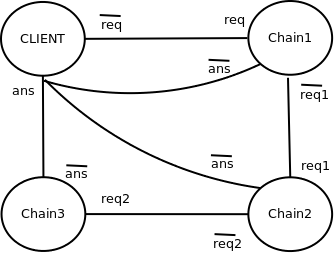
\includegraphics[width=10cm, height=8cm]{screen/Diagram2.png}



\bibliographystyle{plain} 
\nocite{*} \bibliography{myrefs}


\end{document}
